\documentclass[conference]{IEEEtran}

%%%%%%%%%%%%%%%%%%%%%%%%%%%%%%%%%%%%%%%%%%%%%%%%%%%%%%%%%%%%%%%%%%%%%%%%%%%%%%%%
%
% Package
%
%%%%%%%%%%%%%%%%%%%%%%%%%%%%%%%%%%%%%%%%%%%%%%%%%%%%%%%%%%%%%%%%%%%%%%%%%%%%%%%%
\usepackage{ifpdf}
\ifCLASSINFOpdf
  \usepackage[pdftex]{graphicx}
  % declare the path(s) where your graphic files are
  % \graphicspath{{../pdf/}{../jpeg/}}
  % and their extensions so you won't have to specify these with
  % every instance of \includegraphics
  \DeclareGraphicsExtensions{.pdf,.jpeg,.png}
\else
  % or other class option (dvipsone, dvipdf, if not using dvips). graphicx
  % will default to the driver specified in the system graphics.cfg if no
  % driver is specified.
  \usepackage[dvips]{graphicx}
  % declare the path(s) where your graphic files are
  % \graphicspath{{../eps/}}
  % and their extensions so you won't have to specify these with
  % every instance of \includegraphics
  \DeclareGraphicsExtensions{.eps}
\fi

\usepackage[utf8]{inputenc}
\usepackage[T1]{fontenc}
\usepackage[french, english]{babel}
\usepackage{cite}
\usepackage{caption}
\usepackage{amsmath,amsfonts,amssymb}
\usepackage{subcaption}
\usepackage{array}

%
% correct bad hyphenation here
\hyphenation{op-tical net-works semi-conduc-tor}


\begin{document}
%%%%%%%%%%%%%%%%%%%%%%%%%%%%%%%%%%%%%%%%%%%%%%%%%%%%%%%%%%%%%%%%%%%%%%%%%%%%%%%%
%
% Title
%
%%%%%%%%%%%%%%%%%%%%%%%%%%%%%%%%%%%%%%%%%%%%%%%%%%%%%%%%%%%%%%%%%%%%%%%%%%%%%%%%
\title{Coalition Formation Algorithm of Prosumers in a Smart Grid Environment}

%%%%%%%%%%%%%%%%%%%%%%%%%%%%%%%%%%%%%%%%%%%%%%%%%%%%%%%%%%%%%%%%%%%%%%%%%%%%%%%%
%
% Authors
%
%%%%%%%%%%%%%%%%%%%%%%%%%%%%%%%%%%%%%%%%%%%%%%%%%%%%%%%%%%%%%%%%%%%%%%%%%%%%%%%%
\author{Nicolas Gensollen, Vincent Gauthier, Michel Marot and Monique Becker \\
\IEEEauthorblockA{CNRS UMR 5157 SAMOVAR, \\
Telecom SudParis/Institut Mines Telecom\\
Email: \{nicolas.gensollen, vincent.gauthier, michel.marot, monique.becker\}@telecom-sudparis.eu}}

\maketitle

%%%%%%%%%%%%%%%%%%%%%%%%%%%%%%%%%%%%%%%%%%%%%%%%%%%%%%%%%%%%%%%%%%%%%%%%%%%%%%%%
%
% Abstract
%
%%%%%%%%%%%%%%%%%%%%%%%%%%%%%%%%%%%%%%%%%%%%%%%%%%%%%%%%%%%%%%%%%%%%%%%%%%%%%%%%
\begin{abstract}
In a smart grid environment, we study coalition formation of prosumers that aim at selling energy to the grid. It is paramount for the grid operation that the energy producers are able to sustain the grid demand in terms of stability and minimum production requirement in order to enter the energy market. We design an algorithm that seeks to form coalitions that will meet both of these requirements:  a minimum energy level for the coalitions and a steady production level which leads to finding uncorrelated sources of energy  to form a coalition. We propose an algorithm that uses graph tools such as correlation graphs or clique percolation to form coalitions that meet such complex constraints. We validate the algorithm against a random procedure and show that, it not only performs better in term of social welfare for the power grid, but also that it is more robust against unforeseen production variations due to changing weather conditions for instance. 
\end{abstract}

\IEEEpeerreviewmaketitle


%%%%%%%%%%%%%%%%%%%%%%%%%%%%%%%%%%%%%%%%%%%%%%%%%%%%%%%%%%%%%%%%%%%%%%%%%%%%%%%%
%
% Section I: Introduction
%
%%%%%%%%%%%%%%%%%%%%%%%%%%%%%%%%%%%%%%%%%%%%%%%%%%%%%%%%%%%%%%%%%%%%%%%%%%%%%%%%
\section{Introduction}
\label{sec:introduction}

One of the key ideas in the smart grid revolves around the introduction of communication means inside the power grids. This could enable complex improvements in the energy management and lead progressively to a greener energetic system \cite{Ramchurn} \cite{WuHamedHuangBook2011}. Distributed energy resources (DER) such as wind turbines or photovoltaic panels are not supposed to emerge only in remote farms, but also in residential areas. Together with electric vehicles, and demand side management tools, they will constitute the building blocks which will help to turn the today pure energy consumers into true actors of the grid operation \cite{Ramchurn}. Such agents that both consume and produce energy are ready to make concessions (appliances delays, V2G) to ensure grid stability, and are commonly called prosumers \cite{Rathnayaka2012} \cite{Ramchurn}.

There seems to have a clear consensus on the benefit of having bidirectional communication flows between the prosumers and the grid, as most of the demand side management concepts have proposed such an architecture \cite{WuHamedHuangBook2011}. Nevertheless as the number of active prosumers is expected to rise, it is safe to assume there is a need for more complex communication patterns (such as coalitions) that will help to decrease the communication burden and in the mean time satisfy the multiple requirements of the power grid management. The formation of coalitions inside the smart grid environment could be applied to various types of agents such as self sufficient micro-grids \cite{Pahwa}, sizable and adjustable virtual power plants (VPP) \cite{Braun, Ramchurn}, or fleet of electric vehicles that back up the grid in some emergency situations (V2G) \cite{Ramchurn}. These are just a few use cases where the coalition of multiple agents can enhance the grid reliability and in the mean time reduce the communication burden.

In this paper, we focus on how to statistically improve the production stability by carefully forming coalitions of prosumers that have greater probabilities of staying in acceptable range of production. By using prediction techniques, we form coalitions that meet the contract values ranges proposed by the grid, enabling it to schedule its production accordingly. Meeting contract values for the prosumers is especially relevant in power trade conditions, where energy is traded based on day-ahead predictions. In this context, participants should try to minimize their prediction errors in order to maintain a stable state for the grid. They may even occur some penalties if the productions deviate from the initial contract values. However, it remains pertinent for both side to maintain the production as stable as possible : for the prosumer, the stability (with renewable energy sources) will impact its net gain, and for the power grid, it will help to maintain its reliability.

In this paper, we seek to form coalitions that are able to announce "high contract values with high reliability". We thus aim at:
\begin{itemize}
\item Building a realistic prosumer model with renewable production sources based on weather data (see section \ref{subsec:ProsumerModel}).
\item Define a coalition formation model that enables the grid to set some requirements under which any group of prosumers will be allowed to sell its production (see section \ref{subsec:Coalition})
\item Define a utility function that will satisfy the grid requirements and maximize the stability of the prosumer coalition productions (see section \ref{subsec:UtilityFunc})
\item Define a coalition formation algorithm (see section \ref{sec:forming})
\end{itemize}

In section \ref{sec:model}, we consider that the agent's production depend on meteorological conditions (wind turbines and PV as generators), various energy mix and preferences, and their appliances (loads). We use meteorological data (see section \ref{subsec:ProsumerModel}) to account for seasonal and daily variations in the prosumer's energetic profiles as well as realistic geographical correlations between different agents. With these ingredients, we are able to run realistic simulations and record the different output profiles as time-series.

In order to select groups of prosumers that lower the volatility of the coalition's productions, we define an algorithm based on a popular approach for stocks market clustering \cite{Mantegna1999}. We use a modified clique percolation algorithm (see section \ref{sec:forming}) that will enable us to expand the cliques as needed in order to form proper coalitions that fulfill both the grid requirements and lower the production volatility. Finally, section \ref{sec:results} provides some results and a conclusion in section \ref{sec:conclusion}.

%%%%%%%%%%%%%%%%%%%%%%%%%%%%%%%%%%%%%%%%%%%%%%%%%%%%%%%%%%%%%%%%%%%%%%%%%%%%%%%%
%
% Section II: Related Work
%
%%%%%%%%%%%%%%%%%%%%%%%%%%%%%%%%%%%%%%%%%%%%%%%%%%%%%%%%%%%%%%%%%%%%%%%%%%%%%%%%

\section{Related Work}
\label{sec:related}

Traditionally, forming coalitions in a pool of agents can be done either in a centralized way where a single central unit is responsible for all the computations or in a distributed way where agents have only local knowledges and take actions accordingly. It is of common use to represent the situation and assess the stability of the solution by using game theoretic tools. Some papers \cite{Saad2009} \cite{Luan2014} focus then on finding an optimal coalition structure giving a pool of autonomous self interested agents using distributed merge/split algorithms.

Tackling the stability issues of renewable DER, the TradeWind project \cite{Europe} simulated the impact of wind power on electricity exchange and cross-border congestions by using a flow-based market model. The idea revolves around identifying key european interconnections (already existant or not) in order "to make optimal use of the european spacial de-correlation of wind power". It was indeed shown that geographical aggregation provides smoothening effects and that the amount of prediction errors for wind power in a geographical region diminishes as the region size increases, especially for short forecast horizons.

On a narrower scale, the authors of \cite{Kota2011} study the formation of virtual power plants (VPP) composed of multiple self-interested DER. On the grid side, two requirements for the formation of virtual power plants are considered : the reliability of supply and the minimization of entities the grid has to deal with. From this, \cite{Kota2011} builds a pricing mechanism that encourages VPP to report true estimates of their aggregated production and penalizes prediction errors. A redistribution scheme of the VPP to the DER is also constructed such that the payoff allocation lies in the core of the game, meaning that no DER has an incentive to leave the coalition.

In this paper we ought to form coalitions utilities that depend on statistical properties of time-series values. The setting is thus similar with some financial studies on stock exchanges, where researchers tried to find relevant clusters of stocks based on their daily prices variations. The problem of clustering is usually approached by means of a similarity measure and completed by a clustering technique such as K-means or hierarchical clustering. Nevertheless, in \cite{Mantegna1999} the author introduced an approach where stocks time-series of their daily log returns, are organized in a graph such that stocks exhibiting similar price fluctuation patterns are close to each other. This closeness notion is formalized with a similarity measure based on Pearson correlation coefficient ($ d_{ij} = \dfrac{1}{2}\sqrt{2(1-\rho_{ij})} $ or $ d_{ij} = 1 - \rho_{ij}^{2} $ ) that enables to weight the edges of the graph. 

$\epsilon$-graphs, consists in filtering edges based on their weight, only keeping edges whose weights are less than $ \epsilon $. In \cite{Garas2008, Onnela2004}, the authors studied the topological properties (average clustering, connectivity, relative number of cliques) of the correlation graph against those of growing random graphs, depending on the threshold $ \epsilon $. However, there is no well defined method to select of right tradeoff $ \epsilon $ as function of the network topology.

Presented in this way, the time-series clustering task seems very close to graph community detection. Communities in networks are indeed often seen as groups of nodes exhibiting high internal densities of links as well as a low density across communities \cite{Newmanb}. Although several techniques exists (based on different graph properties : modularity \cite{Newmanb}, edge betweenness \cite{Girvan2002}, spectrum of graph Laplacian \cite{Newman}), the clique percolation algorithm \cite{Lancichinetti} uses directly this observation and employs a greedy expansion rule based on a fitness function. When the algorithm stops, some coalitions may be partially overlapping, meaning that a node can belong to multiple communities. Detection of overlapping communities is actually a very active field of research, especially in social networks where a person might belong to several communities in the mean time.

%%%%%%%%%%%%%%%%%%%%%%%%%%%%%%%%%%%%%%%%%%%%%%%%%%%%%%%%%%%%%%%%%%%%%%%%%%%%%%%%
%
% Section III: Model
%
%%%%%%%%%%%%%%%%%%%%%%%%%%%%%%%%%%%%%%%%%%%%%%%%%%%%%%%%%%%%%%%%%%%%%%%%%%%%%%%%

\section{Model}
\label{sec:model}
\subsection{Prosumer model}\label{subsec:ProsumerModel}

Our major concern was to design a prosumer model with realistic patterns of consumption, production as well as realistic geographical correlations between them. We based our prosumer model on French's weather data from 2006 to 2012 sampled every 3 hours \cite{Infoclimat} (similar data are available for the United States covering 2010\cite{NCDC}). 

As shown in the first part of figure 1, the first step consists in discretizing the studied zone around well chosen weather stations and gathering traces for these stations. In this paper, we consider that prosumers can only produce through wind turbines and photovoltaic panels (PV). On the other hand, we built their consumption patterns according to two major cycles :
\begin{itemize}
\item \textbf{Daily cycles} : Consumption is low during night, and higher during the day with two picks in the morning and evening. Some noise is added so that prosumers have similar but not identical cycles.
\item \textbf{Seasonal cycles} : Consumption is higher in the winter because of heating and low in the summer (air conditioning is not considered). Temperature traces were the principal ingredient for modeling these cycles.
\end{itemize} 

\begin{center}
\begin{figure}
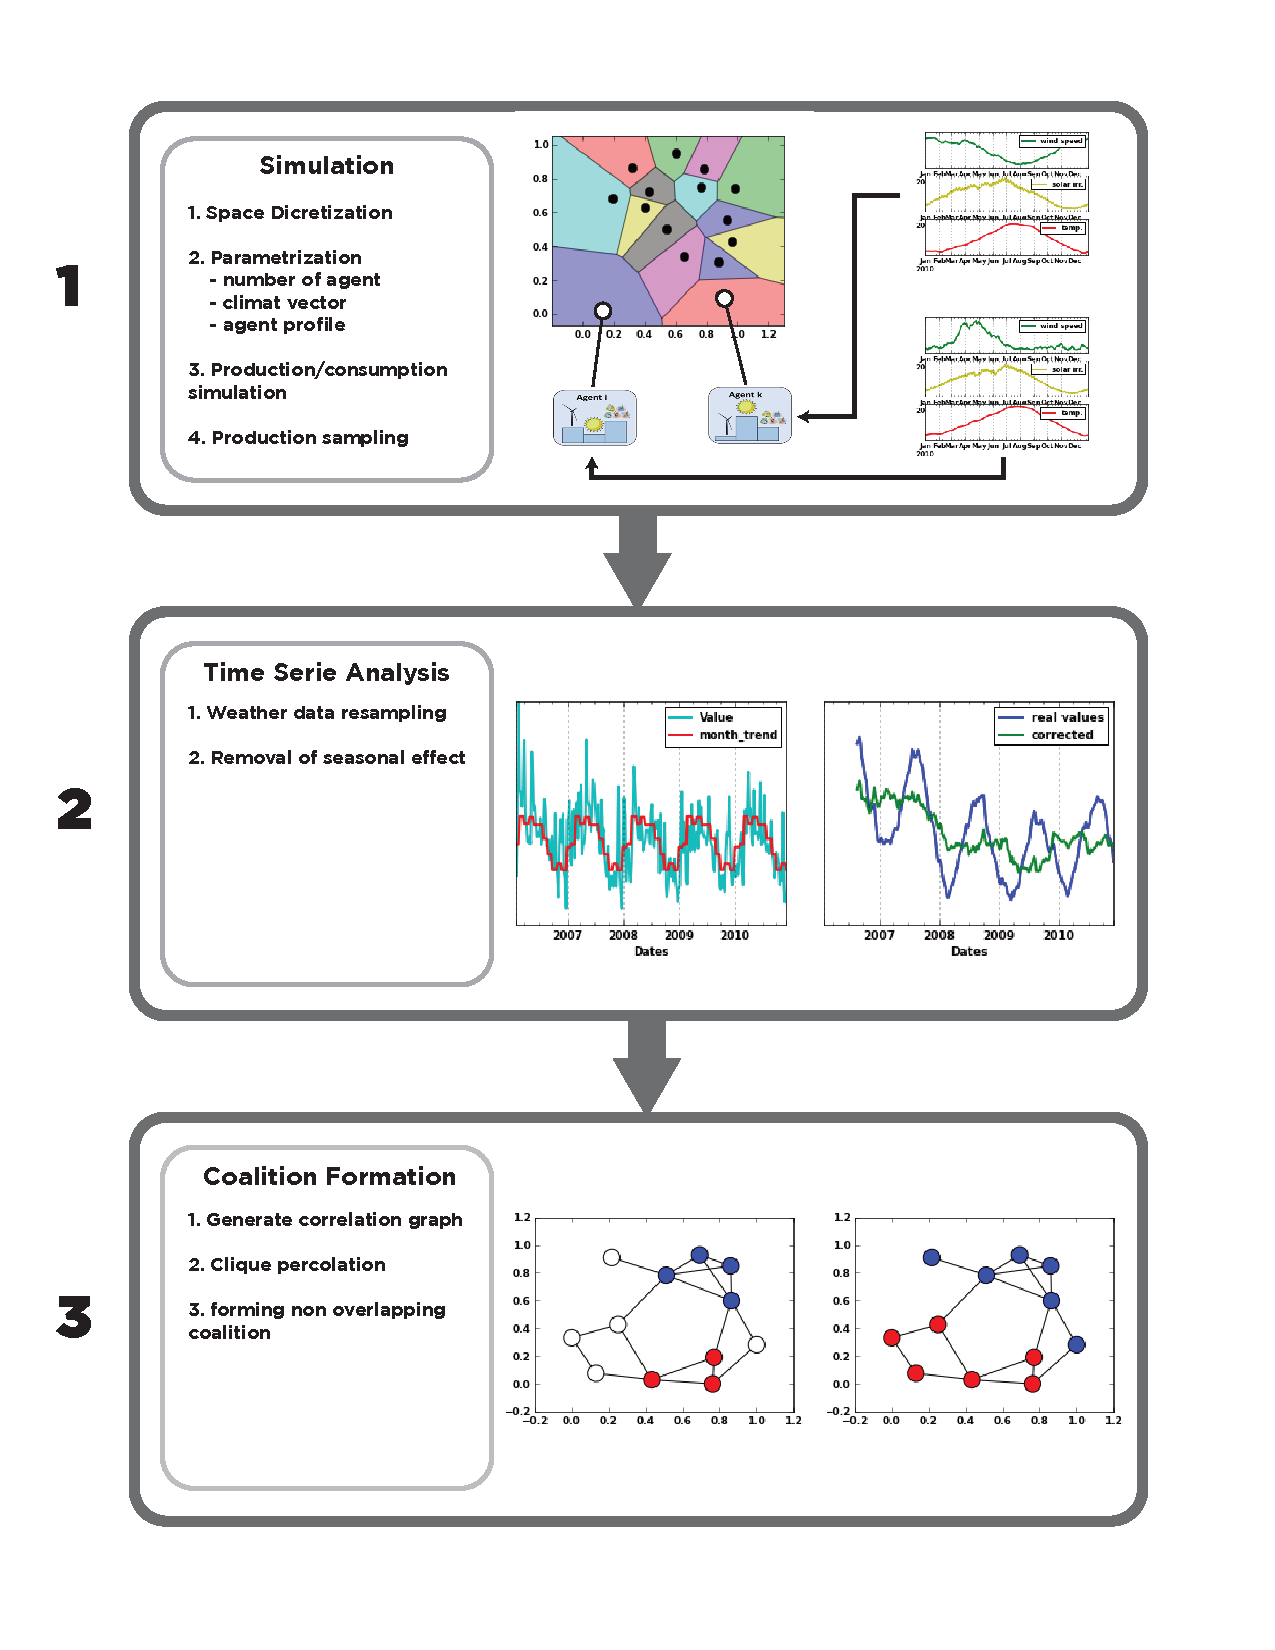
\includegraphics[scale=0.45]{figure2/Fig2}
\caption{Process diagram}
\label{Fig1}
\end{figure}
\end{center}

We thus collect for all chosen weather stations three kinds of data (average wind speed, cloudiness, and average temperature), which we will call a climate vector in the following. We consider that climate vectors are constant over their area, meaning that, if two agents are in the same area, they are exposed to the same climate vector.

At this point, modeling agents consists in fixing a few parameters (most of the time drawn from random distributions) such as the geographical position, the number of wind turbines, PV, appliances, the temperature of confort, and so on. The objective is that, depending on the weather of his zone, the DER and appliances he owns, and the way he decides to heat his home, a given prosumer is able to compute his production/consumption at any time. 

We thus used existing models enabling conversion between weather variables and output powers (see power curves in \cite{Kota2011} \cite{windturbinemodel}). \cite{Dans2007} provides also a convenient way of using cloudiness traces as realistic degradation factors in a \textit{"clear blue sky"} solar model, which enables us to rebuild realistic solar irradiance traces for stations that do not provide such information directly. Any agent is thus able to compute at any time how much he produces and consumes. 

\subsection{Coalition formation model}\label{subsec:Coalition}
More formally, we denote by $ \mathcal{A} = \{ a_{1},...a_{N} \} $ the set of agents (the prosumers) and $ P_{i}(t) $ the instantaneous power value at agent i at instant t (its instantaneous production minus his instantaneous consumption, meaning that $ P_{i}(t) $ represents agent i available power at instant t). During the simulation (from $t_{0} $ to $ t_{K} $), all agents record their values with an hour time interval. As expected (because we introduced them), the time-series exhibit high seasonal patterns, but completely different from agent to agent because they depend both of their energetic mix and habits of a given prosumer. Nevertheless, these macro variations can hide the interesting information in the correlation coefficients and twist the rest of our process. Thereby, we remove these seasonal effects for all agents (see second block of figure \ref{Fig1}). We denote by $ \mathcal{T}_{i} = \{ P_{i}(t_{0}),...,P_{i}(t_{K}) \} $ the resulting time-series for  agent i, and by $ \mathcal{P}_{i} $ the corresponding probability distribution.

We now extend these notations to any coalition $ S \subset \mathcal{A} $ : 
\begin{itemize}
\item $ P_{S}(t) = \sum_{i \in S} P_{i}(t) $
\item $ \mathcal{T}_{S} = \{ P_{S}(t_{0}),...,P_{S}(t_{K}) \} $ with $ \mathcal{P}_{S} $ the corresponding probability distribution
\item A coalition S has the possibility to announce a contract value $ P_{S}^{CRCT} $ on the market.
\end{itemize}

Due to the volatile nature of DER productions or user consumptions, the available power of a coalition will oscillates around $ P_{S}^{CRCT} $. It will be the responsability of the coalition, that is the information system maintaining the coalition, to compensate for deviations. In this paper, we consider then that the smaller these deviations, the better. Based on the $ \mathcal{T}_{S} $ distribution, the probability of S value (at any instant t) being below its contract value $ Pr[P_{S}(t) \leq P_{S}^{CRCT} ] $ appears therefore as a quantity of interest that we would want to keep as low as possible. 

In this model, we consider that only the coalitions that have this probability value sufficiently low are acceptable. That is, we denote by $ \phi \in [0,1] $ the threshold imposed to the coalitions over this quantity, and we call it the \textbf{reliability} in the following. The reliability stipulates then that for any coalition S willing to join the market, the probability of S value (at any instant t) being below its contract value should at most be $ \phi $. That is, $ \forall S,\ \forall t,\ Pr[P_{S}(t) \leq P_{S}^{CRCT} ] \leq \phi $ ($ \phi $ being restricted to small values for consistency).

We then consider another constraint denoted by $ P^{MIN} $, as the \textbf{minimum contract value}, which states that only coalitions with higher contract values ($ P_{S}^{CRCT} \geq P^{MIN} $) will be accepted. Figure \ref{Fig89} summurizes the main notations of this paper.

At this point, if a coalition S wishes to join the market, it has to choose a contract value that fulfill the two conditions. For simplification, we consider that coalitions will always apply the same economically consistent strategy of announcing the highest possible contract value that obeys the reliability rule (a value we denote by $ P_{\phi}(S) $). If $ P_{\phi}(S) \geq P^{MIN} $, meaning that it also obeys the minimum contract value rule, then S announces this value on the market : $ P_{S}^{CRCT} = P_{\phi}(S) $. Otherwise, coalition S is not able to enter.
Basically, a coalition S is valid if and only if :
\begin{equation}
\left\{ \begin{array}{lll}
		\forall t,\ Pr[ P_{S}(t) \leq P_{\phi}(S)] \leq \phi\ \textit{{\scriptsize (reliability rule)}} \\
		and\ P_{\phi}(S) \geq P^{MIN}\ \textit{{\scriptsize (min value rule)}}

\end{array} \right. 
\label{rules}
\end{equation}

\subsection{Utility function}\label{subsec:UtilityFunc}
We now choose a very simple utility function (eq. \ref{utility}) that derives directly from the above remarks. If a coalition cannot provide a valid contract value, it receives naturally a utility of zero. Furthermore, it seems obvious that the utility should increase with the contract value. The $ 1/|S| $ term in eq. \ref{utility} indicates that we favorise small coalitions, mainly because they are easier to maintain in terms of communications.

\begin{equation}
 \mathcal{U}_{\phi,\ P^{MIN}}(S) = \mathbf{1}_{\textit{S\ valid}} \dfrac{P_{\phi}(S)}{|S|} 
\label{utility}
\end{equation}

Obviously, maximising this utility function amounts to maximizing the coalition contract value with the minimum possible number of agents. 

In order to illustrate what is done in the following, lets consider a very simple example with two agents, say i and j, with gaussian value probability distributions $ \mathcal{P}_{i} = \mathcal{N}(\mu_{i}, \sigma_{i}) $ and $ \mathcal{P}_{j} = \mathcal{N}(\mu_{j}, \sigma_{j}) $, such that the joint probability distribution  $ \mathcal{P}_{ij} $ of the coalition $\{ij\}$ is also a gaussian with the following parameters :

\begin{equation}
\left\{ \begin{array}{lll}
		\mu_{ij} = \mu_{i} + \mu_{j} \\
		\sigma_{ij} = \sqrt{\sigma_{i}^{2} + \sigma_{j}^{2} + \rho_{ij}\sigma_{i}\sigma_{j}}
\end{array} \right.
\label{parameters}
\end{equation}

with $ \rho_{ij} $ the Pearson correlation coefficient between $ P_{i} $ and $ P_{j} $. We can easily write the reliability condition $ Pr[P_{ij}(t) \leq P_{\phi}(ij) ] \leq \phi $ as :

\begin{equation}
\dfrac{1}{2} \left[ 1+ erf \left( \dfrac{P_{\phi}(ij) - \mu_{ij}}{\sigma_{ij}\sqrt{2}} \right) \right] \leq \phi
\label{reliability}
\end{equation}

The strategy of $ \{ij\} $ consists in maximizing its contract value as long as it respects the inequality \ref{reliability}, e.g to annonce $ P_{\phi}(ij) = \mu_{ij} - \sigma_{ij}\sqrt{2}erf^{-1}(1-2 \phi ) $. It thus appears (as it was intuitively understandable) that, for equivalent sizes, coalitions with low relative standard deviations ( $ \sigma_{ij} / \mu_{ij} $ ) are able to announce higher contract values. 

What this paper investigates in the following is the developement of an algorithm that organizes prosumers such that the synergy term of the standard deviation ( $ \rho_{ij}\sigma_{i}\sigma_{j} $ in the example above) is minimized. In such settings, and through the clique percolation procedure (section \ref{sec:forming}), we will show that coalitions with low relative standard deviations, e.g high utility coalitions, can be computed.

\begin{table}[!t]
\label{Fig89}
\centering
\scriptsize
\begin{tabular}{l|p{4.5cm}}
  \hline
  \textbf{Symbols} &  \\
  \hline 
  $ \mathcal{A}=\{a_{1},...,a_{N}\} $ & Set of agents \\
  $ P_{i}(t) \in \mathbb{R}\ \ (P_{S}(t)) $ & Instantaneous production of agent $i$ in coalition $S$ at time $t$ \\
  $ \mathcal{T}_{i} = \{P_{i}(t_{0}),...,P_{i}(t_{K})\} $ & Time series of agent i available production values \\
  $ \mathcal{P}_{i}\ \ (\mathcal{P}_{S}) $ & Probability distribution of the production of the agent i in coalition S\\
  $ \phi \in [0,1] $ & Reliability threshold \\
  $ P^{MIN} \in \mathbb{R}^+ $ & Min value threshold \\
  $ P_{S}^{CRCT} \in \mathbb{R}^+ $ & Contract value of coalition S \\
  $ P_{\phi}(S) \in \mathbb{R}^+ $ & Max contract value under $ \phi $ constraint \\
  $ \mathcal{U}_{\phi,\ P^{MIN}}(S) $ & Utility function \\
  $ \tau_{i}(S) \in \mathbb{R}$ & Decision rule for mapping overlapping into disjoint coalitions \\
  $ \epsilon \in [0,1] $ & Pruning threshold for the correlation graph \\
  $ N_{COAL} \in \mathbb{Z}^+ $ & Number of desired coalition \\
  $ CS = \{S_{1},...,S_{N_{COAL}}\} $ & Coalition structure \\
  \hline
\end{tabular}
\caption{Notations}
\end{table}


%%%%%%%%%%%%%%%%%%%%%%%%%%%%%%%%%%%%%%%%%%%%%%%%%%%%%%%%%%%%%%%%%%%%%%%%%%%%%%%%
%
% Section V: Coalition Formation
%
%%%%%%%%%%%%%%%%%%%%%%%%%%%%%%%%%%%%%%%%%%%%%%%%%%%%%%%%%%%%%%%%%%%%%%%%%%%%%%%%

\section{Coalition Formation}
\label{sec:forming}

This section explains the process with which we form the coalitions (see the third block of Figure \ref{Fig1}). First, we need to simulate the timeseries of available power (first two blocks of Figure \ref{Fig1}). We consider a pool $ \mathcal{A} $ of 200 agents, whose parameters were chosen randomly. The prosumers are positioned (also randomly) on a square lattice previously filled with climate vectors obtained from the french data sets (see section \ref{sec:model}). Simulations were run from february 2006 to december 2010 such that we are dealing with 200 hourly sampled timeseries of available power over this period. Removing season trends finally leads us to the formation of coalitions. 

The model we used in order to simulate timeseries of available production provides some diversity because of the combination between the energetic mix and the climate vectors. Nevertheless, as the number of agents grows, the timeseries tend to exhibit similar patterns. This is apparent when creating a correlation graph $ G_{1}(\mathcal{A},E_{1},\omega_{1}) $ with the same kind of metric as \cite{Garas2008} or \cite{Onnela2004} ($ d_{ij} = 1 - \rho_{ij}^{2} $), where well defined clusters appear in the $ \epsilon $-graph for any values of $ \epsilon $. 

However, these clusters of strongly correlated timeseries are the exact opposite of what we are seeking. We can indeed consider them directly as coalitions and compute their utilities, and the results show (see the green curves on figure \ref{Fig4}), as expected, terrible values (far worse than a random split of the agents in the same number of coalitions).

We thus opt for reversing the metric ($ d_{ij}^{'} = \rho_{ij}^{2} $) such that uncorrelated timeseries are close to each other and (anti)correlated timeseries are distant in $ G_{2}(\mathcal{A},E_{2},\omega_{2}) $. As expected \cite{Onnela2004}, independently of the $ \epsilon $ parameter, the resulting $ \epsilon $-graph exhibits henceforth much less clustering than in $ G_{1} $ and communities seem hardly visible. Therefore, using classical clustering or community detection algorithms seem to provide poor results. 

However, as seems intuitively understandable, cliques of this graph tend to exhibit very good utility values. Such  structures contain indeed a link between every two nodes, meaning that the overall correlation is quite small. Obviously, the $ \epsilon $ parameter is indirectly responsible for the sizes of the cliques, if it is too low, the $\epsilon$-graph of $ G_{2} $ will not provide enough cliques, conversely, if $\epsilon $ is too high, we loose important information as the graph becomes very dense and cliques tend to overlap strongly. For large values of $ \epsilon $ and for non trivial number of agents, finding cliques can even become computationally repulsive. Despite being direct and simple, improving the sizes of the cliques by increasing $ \epsilon $ seems too brutal. Furthermore, as the utility function is also focused on maximizing $ P_{\phi}(S) $, it might be the case that some cliques benefit from additional agents even if they don't form a clique anymore.

Cliques for small values of $ \epsilon $ appear thus as good seeds for stable coalitions, but we still have to find a way to bring them above the grid requirements as well as increasing the social welfare, both by incorporating more nodes. This is exactly where clique percolation proves useful for our concerns. The main idea of making the seeds grow as long as it increases a fitness function is exactly what we need. The only difference being that our fitness function is simply chosen as the utility function.  

As explained in section \ref{sec:related}, clique percolation leads generally to overlapping communities. For simplicity, in this paper, we wish to keep the coalitions separated and  leave the management of overlapping coalitions for future work. We thus implemented a simple heuristic that consider nodes in multiple seeds one by one and chooses its final coalition as the one that “needs it the most” in terms of utility loss. More formally, for a coalition S and a node $ i \in S $, we define :

\begin{equation}
\tau_{i}(S) = \dfrac{\mathcal{U}_{\phi,\ P^{MIN}}(S) - \mathcal{U}_{\phi,\ P^{MIN}}(S-\{i\}) }{\mathcal{U}_{\phi,\ P^{MIN}}(S)}
\label{tau}
\end{equation}

If node i belongs to  multiple coalitions, the only coalition retaining node i is the one that maximizes $ \tau_{i} $.

At this point, we have three degrees of freedom : the reliability ($ \phi $), the required power to enter the market ($P^{MIN}$), and the prunning parameter ($\epsilon$). For convenience, we introduce the number of desired coalitions ($ N_{COAL} $) and we fix $\epsilon $ as the smallest value such that the $ \epsilon $-graph contains at least $ N_{COAL} $ non overlaping cliques. The overall utility depends now on the grid requirements and on the number of desired coalitions.

The next section shows how the utility behave within the parameters space and provides the results of our 200 agents test.

\section{Results}
\label{sec:results}

\begin{figure}
 \centering
  \subcaptionbox{$ (\phi, P^{MIN}) $ subspace\label{fig2:a}}{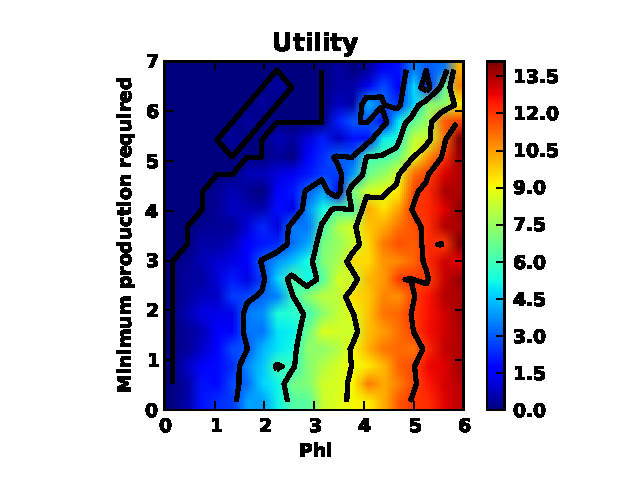
\includegraphics[width=1.7in]{./figure1/util}}
  \subcaptionbox{$ (N_{COAL}, P^{MIN}) $ subspace\label{fig2:b}}{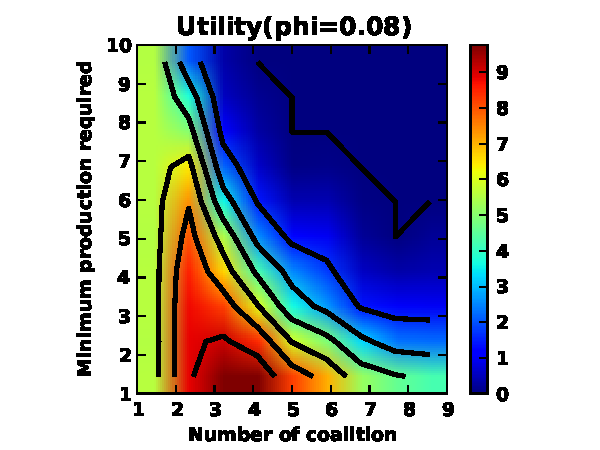
\includegraphics[width=1.70in]{./figure6/util2}}
\caption{Utility function as function of the parameters space $\{\phi \in [0,1], N_{COAL}\in \mathbb{Z}^+, P^{MIN} \in \mathbb{R}^+\}$: In $ \{\phi \in [0,0.6], P^{MIN}\} $ when $ N_{COAL} $ is fixed (fig \ref{fig2:a}), and in $ \{N_{COAL}, P^{MIN}\} $ for a fixed $ \phi $ (fig \ref{fig2:b}). For readability, $ P^{MIN} $ is expressed in tenth of MW.}
\label{Fig2}
\end{figure}

As shown in figure \ref{fig2:a}, the parameters $\phi$ and $P^{MIN}$ shape the utility function such that, if $ \phi $ is close to zero, the reliability requirement is very high. Only small values of $ P^{MIN}$ could then potentially lead to valid coalitions (and positive utility values). Conversely, the higher $\phi$, the less constraints are imposed to the coalitions and more valid coalitions can arise for a larger spectrum of $ P^{MIN}$. Obviously, the highest utility values are found for high $ \phi $, because the coalitions formed are able then to announce higher contract values, yielding higher utilities. 

In figure \ref{fig2:b}, we fix the reliability value to a given empirical value ($\phi = 0.08 $). We can observe how the social welfare $\sum_{S \in CS} \mathcal{U}_{\phi,\ P^{MIN}}(S)$ evolves according to $P^{MIN}$ and $ N_{COAL} = |CS| $. In our setting we can observe  a maximum point around $ N_{COAL} = 3 $, followed by a decrease. There is clearly a maximum number of coalitions sustainable for a given set of parameters. After that point we will form more coalitions that would be unable to pass the grid requirements. Moreover, reckon that increasing $ N_{COAL} $ means also increasing $ \epsilon $, leading to denser graphs, meaning that the algorithm performance will also decrease.

\begin{figure}[htbp]
  \centering
  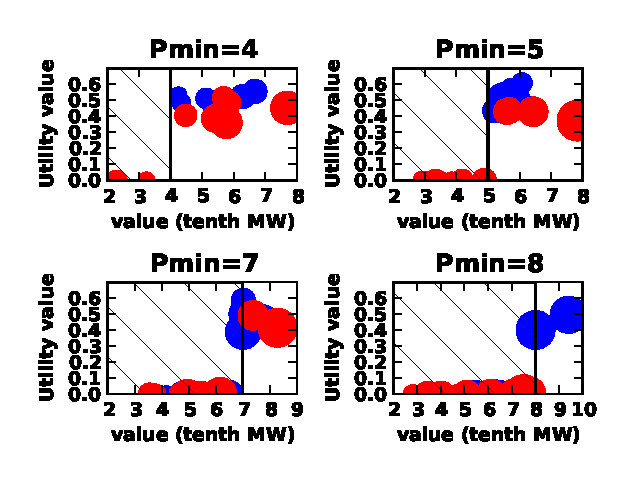
\includegraphics[scale=0.8]{./figure5/coals}
  \caption{Evolution of the coalitions for different values of $ P^{MIN} $ for clique percolation (blue dots) and random process (red dots). The diameters of the dots are proportional to the corresponding coalition sizes. The hatched zone corresponds to the \textit{"under-requirement space"}, and results in zero utility for any coalition in this area.}
  \label{Fig3}
\end{figure}

In figure \ref{Fig3}, we perform a simulation with 200 prosumers, and we fix the reliability $ \phi = 0.1 $ meaning that coalitions should produce more than their contract values at least $ 90 \% $ of the time. We observe the result of our algorithm for a fixed number of coalitions of $N_{coal} = 10$ and let the algorithm form the coalitions as the grid changes according to $ P^{MIN} $. We compare our algorithm with a random process that splits the agents in $ N_{COAL} $ coalitions. Figure \ref{Fig3} shows this evolution for our algorithm (blue dots) and for the random process (red dots). The diameter of a dot is proportional to the number of agents in the coalition and the higher the dot is, the higher its utility. The $ P^{MIN} $ values of the x axis are expressed in tenth of MW for readability and the hatched zone corresponds to the \textit{"under-requirement space"}, meaning that whenever a coalition is in this zone, it has a null utility. 

Looking at figure \ref{Fig3}, we can see first that our algorithm performs better at finding high valued coalitions. The blue dots allowed to enter the market (non hatched zone) are indeed outnumbering the red dots, especially when the grid requirements are neither too low nor too high ($ P^{MIN} = 5 $ in figure \ref{Fig3}).

In more details, figure \ref{fig4:a} presents the evolution of social welfare as the number of coalitions increases (all other parameters are kept constant) for random (red curve), clique percolation (blue curve), and correlated coalitions (green curves) that stands for a worst case scenario. As for figure \ref{fig4:b}, it shows the percentage of coalitions able to enter the market for different values of $ P^{MIN} $. For consistency, we average the results of both plots of the random procedure over 100 realizations.

When the grid requirements are constant (figure \ref{fig4:b}), and the number of desired coalitions is low, clique percolation generally performs better than random case. Moreover, when $ N_{COAL} $ gets bigger, the performance of a random split tumble down rapidly while our clique percolation is able to maintain efficiently the social welfare of the coalitions formed.

When the grid requirements vary, for very low $ P^{MIN} $, all coalitions for all algorithms are able to enter the market, yielding an acceptance percentage of $ 100 \% $. But as $ P^{MIN} $ increases, we see the percentage of the correlated coalitions is going down very quickly. After a few increases in $ P^{MIN} $, the percentage of the random procedure starts dropping while it stays almost constant for our algorithm. For $ P^{MIN} = 8 $, we see that only a little more than half of the coalitions for the random case are able to enter while approximately $ 85 \%$ of them enters for the clique percolation algorithm. Finally, when the grid requirements becomes too high, the acceptance percentage of our algorithm tends slowly to zero (not shown in this plot for readability).


\begin{figure}
 \centering
  \subcaptionbox{Social Welfare\label{fig4:a}}{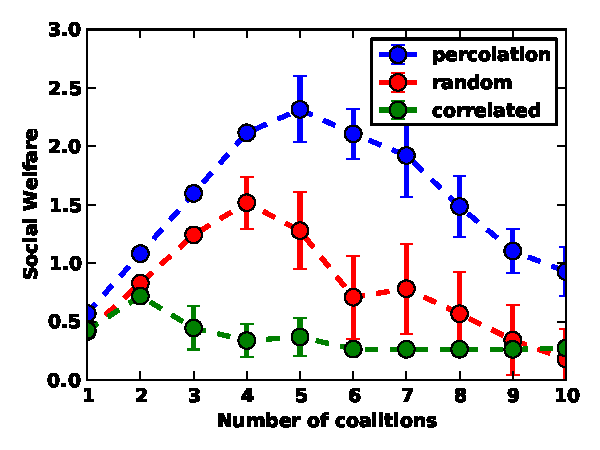
\includegraphics[width=1.6in]{figure7_with_green_curve_v1/uti5}}\hspace{1em}%
  \subcaptionbox{Market entering percentage\label{fig4:b}}{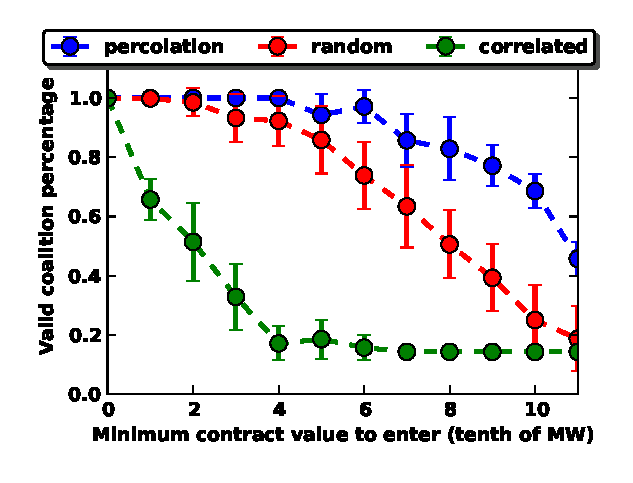
\includegraphics[width=1.6in]{figure4_with_green_curve/survival2_old}}
\caption{Evolution of the social welfare \textbf{a)} and the percentage of coalitions able to enter the market \textbf{b)} for different values of $ P_{MIN} $. Blue curves represent clique percolation, red curves, the random process, and the green ones, correlated coalitions.}
\label{Fig4}
\end{figure}


%%%%%%%%%%%%%%%%%%%%%%%%%%%%%%%%%%%%%%%%%%%%%%%%%%%%%%%%%%%%%%%%%%%%%%%%%%%%%%%%
%
% Section VI: Conclusion
%
%%%%%%%%%%%%%%%%%%%%%%%%%%%%%%%%%%%%%%%%%%%%%%%%%%%%%%%%%%%%%%%%%%%%%%%%%%%%%%%%
\section{Conclusion}
\label{sec:conclusion}

We believe that the originality of this paper lies in its willingness to exploit the de-correlation of prosumer profiles in order to build stable coalitions. In this direction, we presented a model based on meteorological traces, that captures the complex "\textit{energetic mix/climate vectors}" combination and generates realistic production and consumption patterns. We then built a framework that enables the grid to specify stability and minimum production requirements for filtering the coalitions. On this basis, we proposed a simple algorithm that seeks for uncorrelated prosumer patterns as potential seeds and expand them in coalitions able to rise above the grid requirements.

The algorithm is validated against a random process, where we show that it performs better (coalitions are more stable and the overall production is more important) and that it exhibits a higher robustness/flexibility against grid requirements changes.

Interesting leads for future works would be the use of correlated clusters to reduce the number of entities the algorithm has to deal with, or the introduction of a payoff allocation towards the prosumers such that the stability against player defection could be analyzed through game theory. Showing that maintaining the coalitions formed with our algorithm necessitates less communication and less storage capacity could also conduct to a stimulating project. Besides, we believe that not restricting the algorithm to non overlapping coalitions and studying the strategies and weights of nodes with multiple options could lead to interesting works.



%%%%%%%%%%%%%%%%%%%%%%%%%%%%%%%%%%%%%%%%%%%%%%%%%%%%%%%%%%%%%%%%%%%%%%%%%%%%%%%%
%
% Bibliography
%
%%%%%%%%%%%%%%%%%%%%%%%%%%%%%%%%%%%%%%%%%%%%%%%%%%%%%%%%%%%%%%%%%%%%%%%%%%%%%%%%
 
\bibliographystyle{IEEEtran}  
\bibliography{Article}
\end{document}


